% Template for PLoS
% Version 3.5 March 2018
%
% % % % % % % % % % % % % % % % % % % % % %
%
% -- IMPORTANT NOTE
%
% This template contains comments intended 
% to minimize problems and delays during our production 
% process. Please follow the template instructions
% whenever possible.
%
% % % % % % % % % % % % % % % % % % % % % % % 
%
% Once your paper is accepted for publication, 
% PLEASE REMOVE ALL TRACKED CHANGES in this file 
% and leave only the final text of your manuscript. 
% PLOS recommends the use of latexdiff to track changes during review, as this will help to maintain a clean tex file.
% Visit https://www.ctan.org/pkg/latexdiff?lang=en for info or contact us at latex@plos.org.
%
%
% There are no restrictions on package use within the LaTeX files except that 
% no packages listed in the template may be deleted.
%
% Please do not include colors or graphics in the text.
%
% The manuscript LaTeX source should be contained within a single file (do not use \input, \externaldocument, or similar commands).
%
% % % % % % % % % % % % % % % % % % % % % % %
%
% -- FIGURES AND TABLES
%
% Please include tables/figure captions directly after the paragraph where they are first cited in the text.
%
% DO NOT INCLUDE GRAPHICS IN YOUR MANUSCRIPT
% - Figures should be uploaded separately from your manuscript file. 
% - Figures generated using LaTeX should be extracted and removed from the PDF before submission. 
% - Figures containing multiple panels/subfigures must be combined into one image file before submission.
% For figure citations, please use "Fig" instead of "Figure".
% See http://journals.plos.org/plosone/s/figures for PLOS figure guidelines.
%
% Tables should be cell-based and may not contain:
% - spacing/line breaks within cells to alter layout or alignment
% - do not nest tabular environments (no tabular environments within tabular environments)
% - no graphics or colored text (cell background color/shading OK)
% See http://journals.plos.org/plosone/s/tables for table guidelines.
%
% For tables that exceed the width of the text column, use the adjustwidth environment as illustrated in the example table in text below.
%
% % % % % % % % % % % % % % % % % % % % % % % %
%
% -- EQUATIONS, MATH SYMBOLS, SUBSCRIPTS, AND SUPERSCRIPTS
%
% IMPORTANT
% Below are a few tips to help format your equations and other special characters according to our specifications. For more tips to help reduce the possibility of formatting errors during conversion, please see our LaTeX guidelines at http://journals.plos.org/plosone/s/latex
%
% For inline equations, please be sure to include all portions of an equation in the math environment.  For example, x$^2$ is incorrect; this should be formatted as $x^2$ (or $\mathrm{x}^2$ if the romanized font is desired).
%
% Do not include text that is not math in the math environment. For example, CO2 should be written as CO\textsubscript{2} instead of CO$_2$.
%
% Please add line breaks to long display equations when possible in order to fit size of the column. 
%
% For inline equations, please do not include punctuation (commas, etc) within the math environment unless this is part of the equation.
%
% When adding superscript or subscripts outside of brackets/braces, please group using {}.  For example, change "[U(D,E,\gamma)]^2" to "{[U(D,E,\gamma)]}^2". 
%
% Do not use \cal for caligraphic font.  Instead, use \mathcal{}
%
% % % % % % % % % % % % % % % % % % % % % % % % 
%
% Please contact latex@plos.org with any questions.
%
% % % % % % % % % % % % % % % % % % % % % % % %

\documentclass[10pt,letterpaper]{article}
\usepackage[top=0.85in,left=2.75in,footskip=0.75in]{geometry}

% amsmath and amssymb packages, useful for mathematical formulas and symbols
\usepackage{amsmath,amssymb}

% Use adjustwidth environment to exceed column width (see example table in text)
\usepackage{changepage}

% Use Unicode characters when possible
\usepackage[utf8x]{inputenc}

% textcomp package and marvosym package for additional characters
\usepackage{textcomp,marvosym}

% cite package, to clean up citations in the main text. Do not remove.
\usepackage{cite}

% Use nameref to cite supporting information files (see Supporting Information section for more info)
\usepackage{nameref,hyperref}

% line numbers
\usepackage[right]{lineno}

% ligatures disabled
\usepackage{microtype}
\DisableLigatures[f]{encoding = *, family = * }

% color can be used to apply background shading to table cells only
\usepackage[table,dvipsnames]{xcolor}

% array package and thick rules for tables
\usepackage{array}

%strikethrough
\usepackage{soul}

%sara: for commenting the pdf to add alt text (if anyone knows a better solution for atl text please help)
\usepackage{pdfcomment}

%Janani: for inserting sparingly few super relevant emojis
\usepackage{emoji} %Rocio: https://www.overleaf.com/learn/latex/Questions/Inserting_emojis_in_LaTeX_documents_on_Overleaf#Emoji_characters_and_the_Overleaf_editor

% create "+" rule type for thick vertical lines
\newcolumntype{+}{!{\vrule width 2pt}}

% create \thickcline for thick horizontal lines of variable length
\newlength\savedwidth
\newcommand\thickcline[1]{%
  \noalign{\global\savedwidth\arrayrulewidth\global\arrayrulewidth 2pt}%
  \cline{#1}%
  \noalign{\vskip\arrayrulewidth}%
  \noalign{\global\arrayrulewidth\savedwidth}%
}

% \thickhline command for thick horizontal lines that span the table
\newcommand\thickhline{\noalign{\global\savedwidth\arrayrulewidth\global\arrayrulewidth 2pt}%
\hline
\noalign{\global\arrayrulewidth\savedwidth}}


% Remove comment for double spacing
%\usepackage{setspace} 
%\doublespacing

% Text layout
\raggedright
\setlength{\parindent}{0.5cm}
\textwidth 5.25in 
\textheight 8.75in

% Bold the 'Figure #' in the caption and separate it from the title/caption with a period
% Captions will be left justified
\usepackage[aboveskip=1pt,labelfont=bf,labelsep=period,justification=raggedright,singlelinecheck=off]{caption}
\renewcommand{\figurename}{Fig}

% Use the PLoS provided BiBTeX style
\bibliographystyle{plos2015}

% Remove brackets from numbering in List of References
\makeatletter
\renewcommand{\@biblabel}[1]{\quad#1.}
\makeatother



% Header and Footer with logo
\usepackage{lastpage,fancyhdr,graphicx}
\usepackage{epstopdf}
%\pagestyle{myheadings}
\pagestyle{fancy}
\fancyhf{}
%\setlength{\headheight}{27.023pt}
%\lhead{\includegraphics[width=2.0in]{PLOS-submission.eps}}
\rfoot{\thepage/\pageref{LastPage}}
\renewcommand{\headrulewidth}{0pt}
\renewcommand{\footrule}{\hrule height 2pt \vspace{2mm}}
\fancyheadoffset[L]{2.25in}
\fancyfootoffset[L]{2.25in}
\lfoot{\today}

%% Include all macros below

\newcommand{\lorem}{{\bf LOREM}}
\newcommand{\ipsum}{{\bf IPSUM}}

%% END MACROS SECTION


\begin{document}

\vspace*{0.2in}

% Title must be 250 characters or less.
\begin{flushleft}
{\Large
\textbf\newline{Ten simple rules to host an inclusive conference} % Please use "sentence case" for title and headings (capitalize only the first word in a title (or heading), the first word in a subtitle (or subheading), and any proper nouns).
}
\newline
% Insert author names, affiliations and corresponding author email (do not include titles, positions, or degrees).
\\
Rocío Joo\textsuperscript{1*\Yinyang}, 
Andrea Sánchez-Tapia\textsuperscript{2\Yinyang},
Sara Mortara\textsuperscript{3},
Yanina Bellini Saibene\textsuperscript{4},
Heather Turner\textsuperscript{5}, %\ddag},
Dorothea Hug Peter\textsuperscript{6}, %\ddag},
Matt Bannert\textsuperscript{7},
Batool Almazrouq\textsuperscript{8,9},
Liz Hare\textsuperscript{10},
Laura Ación\textsuperscript{11},
Juan Pablo Narváez-Gómez\textsuperscript{12},
Marcela Alfaro Córdoba\textsuperscript{13},
Federico Marini\textsuperscript{14},
Rita Giordano\textsuperscript{15},
Natalia Morandeira\textsuperscript{16},
Adithi Upadhya\textsuperscript{17},
Joselyn Chávez\textsuperscript{18},
Anicet Ebou\textsuperscript{19},
Silvia Canelón\textsuperscript{20},
Janani Ravi\textsuperscript{21}
%,3\textcurrency}
\\
\bigskip
\textbf{1} Global Fishing Watch, Washington, DC 20036, USA
\\
\textbf{2} Affiliation Dept/Program/Center, Institution Name, City, State, Country
\\
\textbf{3} Affiliation Dept/Program/Center, Institution Name, City, State, Country
\\
\textbf{4} Affiliation Dept/Program/Center, Institution Name, City, State, Country
\\
\textbf{5} Department of Statistics, University of Warwick, Coventry, UK
\\
\textbf{6} Affiliation Dept/Program/Center, Institution Name, City, State, Country
\\
\textbf{7} Affiliation Dept/Program/Center, Institution Name, City, State, Country
\\
\textbf{8} Institute of Systems, Molecular and Integrative Biology, University of Liverpool, Liverpool, L69 7ZB, UK
\\
\textbf{9} King Abdullah International Medical Research Center, Riyadh, Saudi Arabia
\\
\textbf{10} Affiliation Dept/Program/Center, Institution Name, City, State, Country
\\
\textbf{11} Affiliation Dept/Program/Center, Institution Name, City, State, Country
\\
\textbf{12} Affiliation Dept/Program/Center, Institution Name, City, State, Country
\\
\textbf{13} Department of Statistics, University of California, Santa Cruz, CA, USA
\\
\textbf{14} Affiliation Dept/Program/Center, Institution Name, City, State, Country
\\
\textbf{15} Affiliation Dept/Program/Center, Institution Name, City, State, Country
\\
\textbf{16} Affiliation Dept/Program/Center, Institution Name, City, State, Country
\\
\textbf{17} ILK Labs/Bengaluru, India - 560046
\\
\textbf{17} Affiliation Dept/Program/Center, Institution Name, City, State, Country
\\
\textbf{19} Bioinformatic team, Département de Formation et de Recherches en Agriculture et Ressources Animales, Institut National Polytechnique Félix Houphouët-Boigny, BP 1313 Yamoussoukro, Côte d’Ivoire.
\\
\textbf{20} Affiliation Dept/Program/Center, Institution Name, City, State, Country
\\
\textbf{21} Departments of Pathobiology and Diagnostic Investigation, Microbiology and Molecular Genetics, Michigan State University, East Lansing, MI 48824, USA
\\
\bigskip

% Insert additional author notes using the symbols described below. Insert symbol callouts after author names as necessary.
% 
% Remove or comment out the author notes below if they aren't used.
%
% Primary Equal Contribution Note
\Yinyang These authors share first authorship of this work.

% Additional Equal Contribution Note
% Also use this double-dagger symbol for special authorship notes, such as senior authorship.
% \ddag These authors also contributed equally to this work.

% Current address notes
% \textcurrency Current Address: Dept/Program/Center, Institution Name, City, State, Country % change symbol to "\textcurrency a" if more than one current address note
% \textcurrency b Insert second current address 
% \textcurrency c Insert third current address

% Deceased author note
% \dag Deceased

% Use the asterisk to denote corresponding authorship and provide email address in note below.
* rocio.joo@globalfishingwatch.org

\end{flushleft}
% Please keep the abstract below 300 words
\section*{Abstract}

Conferences are spaces to meet and network within an academic or technical field, to learn about new advances, and share our work. They can help define career paths and create long-lasting collaborations and opportunities. 
However, these opportunities are not equal for all. 
This article introduces 10 simple rules to host an inclusive conference. 
The authors recently organized the 2021 edition of the useR! statistical computing conference, attracting a broad range of participants from academia, industry, government, and the non-profit sector. 
Coming from different backgrounds, career stages, and even continents, we embraced the challenge of organizing a high-quality virtual conference in the context of the COVID-19 pandemic and making it a kind, inclusive, and accessible experience for as many people as possible.
The rules result from our lessons learned before, during, and after the organization of the conference. 
They have been mainly written for potential organizers or selection committees of conferences, and contain multiple practical tips so that they can help diverse types of events to become as accessible and inclusive as they can and should be.


% % Please keep the Author Summary between 150 and 200 words

\linenumbers

\section*{Introduction}

% Conferences are great, but only for some
Conferences are spaces to meet and reconnect with members from a specific community, learn about advances in the field, and share our recent contributions.
A good conference experience can make a difference in the professional development of the participants and create long-lasting collaborations and opportunities. 
However, opportunities for participating in conferences are not equal for all. 
Many academic and tech conferences have become spaces that reproduce systemic inequalities, by failing to eliminate the barriers for participation and giving more opportunities to the most privileged individuals (typically white people from rich countries, prestigious institutions, native English speakers with no physical disabilities, for example) \cite{arendDisparityConferenceRegistration2019, biggsAcademicConferenceChilly2018, depickerRethinkingInclusionDisability2020a, irishIncreasingParticipationUsing2020}.
The authors of this article have experienced these inequalities in conferences, from different perspectives and levels of inclusion/exclusion and privilege.
We had the opportunity to organize a virtual and global statistical computing conference, useR! 2021 \cite{sanchez-tapia_user_2021-2}, for users and developers of the R programming language \cite{r_core_team_2021}.
Coming from different backgrounds, career stages, and even continents, we embraced the challenge of organizing a high-quality virtual conference in the context of the COVID-19 pandemic and making it a kind, inclusive, and accessible experience for as many people as possible.

% Roadmap of the paper
The rules result from our lessons learned before, during, and after the organization of the useR! conference. 
They are organized in three sections: three pillars, six design rules, and a continuity rule (\textbf{Fig. \ref{fig:diagram}}).
\textbf{The pillars} comprise fundamental rules with key elements to conceive the work on diversity and inclusion in any conference. 
\textbf{Rule 1} is about setting a vision of diversity and inclusion that should guide all the efforts and decision making in the organization.
\textbf{Rule 2} focuses on how to create a safe and welcoming environment for all the attendees. 
\textbf{Rule 3} highlights the importance of starting with an inclusive and diverse organizing team and provides tips on work dynamics.
The \textbf{design rules} focus on weaving inclusion into the conference design process.
In \textbf{Rule 4}, we introduce multiple ways to counteract bias in the conference program (keynotes, program committee, abstract selection, and other spaces). 
\textbf{Rule 5} provides advice for designing an inclusive online component in virtual and hybrid conferences.
\textbf{Rule 6} focuses on accessibility practices to include people with disabilities.
In \textbf{Rule 7}, we provide suggestions to encourage and ensure full participation of non-native English speakers. 
\textbf{Rule 8} provides tips for developing an inclusive communication strategy. 
In \textbf{Rule 9}, we address budgeting for inclusive practices and helping participants with affordable registration costs, scholarships, and other forms of financial support.
Finally, 
a \textbf{continuity Rule} emphasizes the importance of self-assessment and advocates for making the conference part of a long-term commitment to inclusion. 

We believe that these rules will greatly benefit organizers who intend to put inclusion at the core of their conference right from the conception and planning phases.
The rules will also help people who are part of meeting committees that oversee the site/location selection process, or that coordinate with the local organizers of conferences. 
We have designed them for wide adoption to help scientific and technical conferences to become as accessible and inclusive as they can and should be.


% refs for past works in case we add them in line 311.
% %timperleyHeMoanaPukepuke2020, gewinWhatScientistsShould2019, brownAbleismAcademiaWhere2018, marks2021meeting
% some proposals for more inclusive conferences have been put into practice \cite{gichoraTenSimpleRules2010a, levitisCenteringInclusivityDesign2021, atkinsonJournalMedicine20202021, foramittiVirtuesVirtualConferences2021, ninerBetterWhomLeveling2021, rabyMovingAcademicConferences2021, numfocus_discover_2021},


\begin{figure}[!h]
\centering
%ast: use Adobe Acrobat to add missing accessibility metadata to your PDF file. let's try not to forget this when submitting - some edits to the PDF may be needed to add alt-text to the final version https://chi2021.acm.org/for-authors/presenting/papers/guide-to-an-accessible-submission#late
\pdftooltip{
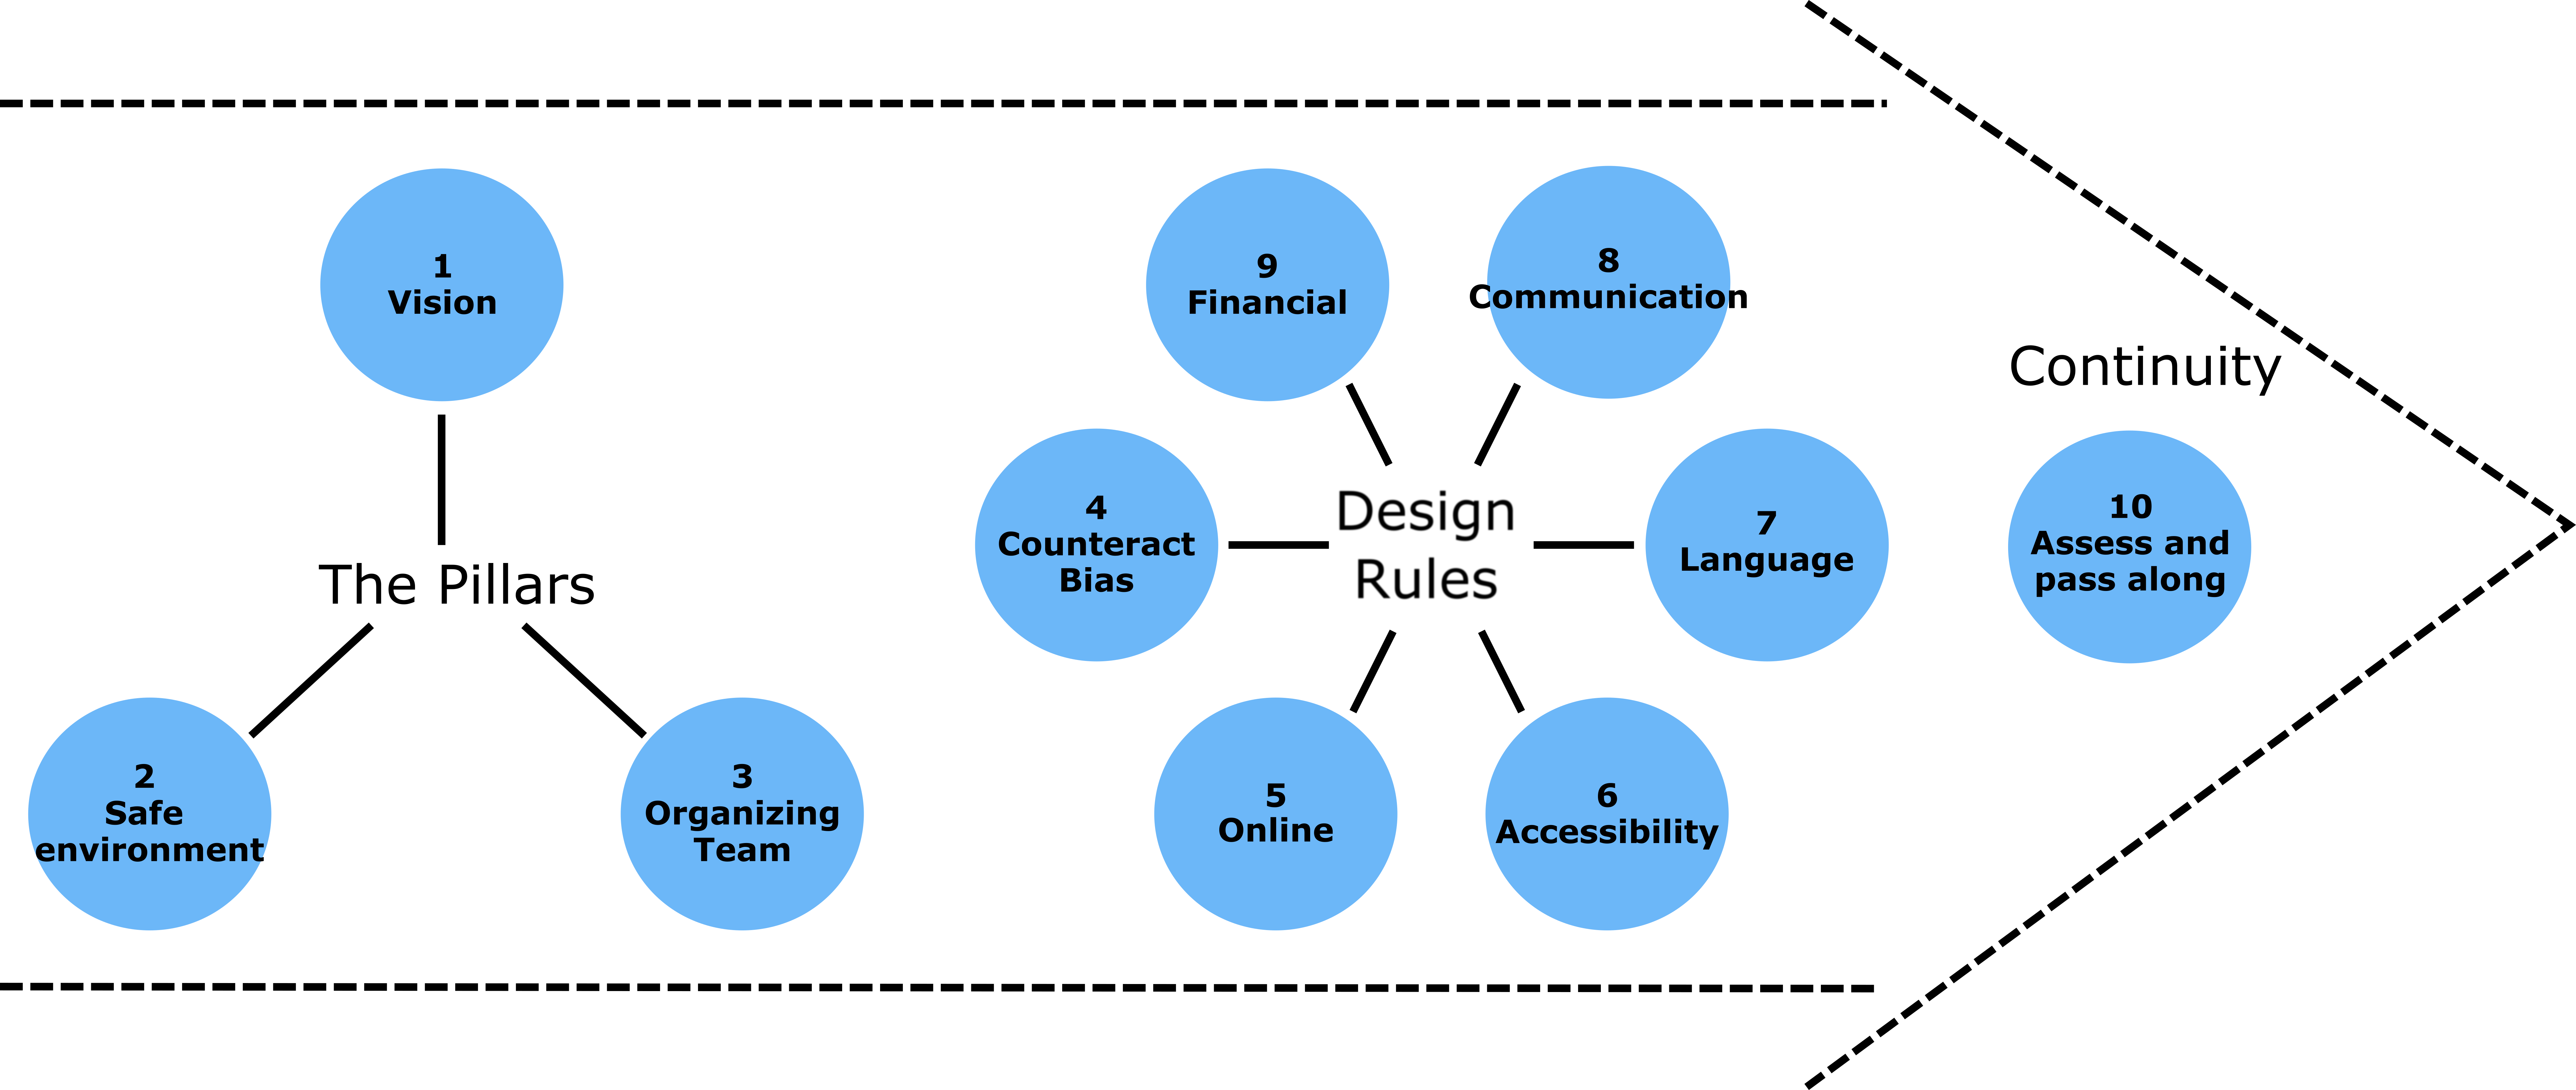
\includegraphics[width=\textwidth]{figs/rules.png}}{
%Alt-text for the figure to be included in the final PDF: Diagram of how the 10 rules are organized into three groups: pillar rules (rules 1-3), design rules (rules 4 to 9), and a continuity rule (rule 10). The overall diagram depicts an arrow from left to right which contains all the rules. From left to right, "the pillars" label is surrounded by blue bubbles which show Rule "1 Vision", Rule "2 Safe environment", and Rule "3 Organizing Team". Then, the label "Design Rules" is surrounded by six blue bubbles with Rules "4 Counteract bias", "5 Online", "6 Accessibility", "7 Language", "8 Communication",  "9 Financial". To the right, and forming the head of the arrow, the Tenth Rule is under the label "Continuity" and consists of a blue bubble "10 Assess and pass along".
}
\caption{Schematic diagram of the rules organized in three groups: the pillars (Rules 1, 2, and 3), design rules (Rules 4 to 9), and continuity (Rule 10).}
\label{fig:diagram}
\end{figure}




\subsection*{Rule 1: Set a vision for diversity and inclusion}
\label{rule_diversity}

Diversity encompasses multiple dimensions: age, physical ability, career stage, gender, gender identity, geographic origin, language, neurodiversity, race, religion, sexual orientation, and socioeconomic background, to name a few.
Human diversity should be celebrated and respected in every way. 
Nonetheless, we live in a world with implicit hierarchies along these axes. 
Some statuses (e.g. being cisgender, white, male, from North America or Western Europe) hold the privilege of being the defaults around which all systems—including conferences—are consciously and unconsciously built. 
People outside the dominant groups suffer different forms of oppression, like sexism, racism, ableism, homophobia, and transphobia, and sometimes these forms of oppression happen simultaneously and in complex ways.
As a result, some groups of people have been systematically excluded from or only partially included in academia and scientific and professional circles.
Recognizing this systematic exclusion is paramount to inclusion.
Assess how it translates to your particular field and scientific or professional community and use this assessment to set the vision and goals of diversity and inclusion for your conference.
Define measurable indicators for these goals (e.g. a gender distribution of your speakers that is representative of the general population, the participation of people from diverse races and ethnicities among the organizers, speakers, and attendees, or participation from key geographic regions) that will help you be accountable along the way.
The vision can be expressed in a diversity statement to be used as a reference for decision making in all areas of the conference organization. 

\subsection*{Rule 2: Create a safe and welcoming environment}
\label{rule_inclusion}

% Inclusion for everyone
% Explain why we need this
Real inclusion can only be achieved in an environment where everybody feels safe, respected, and invited to take part of the conference activities and community. Be proactive and design a welcoming conference experience that takes into account the well-being of all the attendees. This means respecting all the aspects you committed to in your diversity vision (see \textbf{Rule 1}). For example, promote the use and respect of preferred pronouns and commit to respect all genders and sexual orientations. If the conference has an in-person component, pre-assign quiet, private spaces for religious practices, lactation, and child care. Include menu options that account for diverse dietary and religious requirements.
Some of these actions are very easy to implement and have a significant impact on making everyone feel truly included (see \cite{numfocus_discover_2021} for more examples and  great advice on `low-hanging fruits').
Open the schedule for events organized by thematic groups and communities (e.g. taskforce meetings, LGBTQIA+-friendly spaces, Black in STEM), and sessions aimed to welcome first-timers to the conference.

% A culture of support (active bystandership) and code of conduct for a safe place 
Creating a safe and welcoming environment also requires promoting a culture of support, including the idea that anyone can intervene respectfully in defense of other attendees in case anything unpleasant, incorrect, or offensive happens.
This is called `active bystandership'; consider providing training or pre-conference discussions to promote it.
However, the most important step that you should take to ensure the safety of the community is
adopting a code of conduct (CoC) and preparing a diverse response team to enforce it \cite{favaroYourScienceConference2016}.
The CoC is a living document meant to keep the community safe and should state clearly the unacceptable behaviors, the consequences for engaging in such behaviors, and the way to report violations \cite{auroraHowRespondCode2019}.
The CoC response team must receive training on how to receive reports, respond to incidents, and communicate their responses to the whole community. The team should be prepared early during conference planning because CoC violations can happen before the conference too (e.g. social media, organization meetings).  
We strongly recommend reading `How to Respond to code of conduct Reports' \cite{auroraHowRespondCode2019} as an excellent starting point for building a strong CoC response team.
 

\subsection*{Rule 3: Have an inclusive and diverse organizing team}
\label{rule_organizing_team}

% Build a diverse team, and representation
A genuinely inclusive conference can only be organized by an inclusive and diverse team.
Organizers should comprise a team with people from as many different backgrounds as possible regarding regions, genders, ethnicities, career stages, and other aspects of diversity.
People with disabilities often say: `Nothing about us without us' \cite{charlton_nothing_1998, werner_nothing_1998}; the same holds for other dimensions of diversity. 
Having people from diverse backgrounds in decision-making roles will positively affect the conference as a whole because all the processes will benefit from their expertise, experience, and distinct perspectives \cite{hongGroupsDiverseProblem2004}. 
The experience of people in marginalized groups
is especially important; they cannot be replaced by good intentions or second-hand knowledge from people who have not lived through the same experiences \cite{costanzachockDesign2020}.
In addition, a diverse team plays an essential role in creating a welcoming space because representation—seeing people with similar life experiences occupy critical positions of power and breaking negative stereotypes—is one of the best ways to create a sense of belonging for everyone participating in the conference.
It is important, though, to ensure that organizers with diverse backgrounds are not restricted to only work on diversity and inclusion aspects; 
every member should have the freedom to choose which areas of the conference they want to contribute to.

% Rocío: Idea of this paragraph: tips to make a diverse and inclusive team work + paying them
If you have already started assembling an organizing team, check for gaps in its composition and do your best to fill them. 
The regional and local communities, groups, or associations in your field are good sources to tap into. 
When it comes to team leadership, do not expect self-nomination and voting to work as infallible mechanisms to fill these positions equitably. 
People from underrepresented groups sometimes refrain to nominate themselves while people in dominant groups tend to do it more easily. 
Instead, nominate folks directly and offer them leading positions in the organization team, especially those positions that would be typically occupied by people from privileged groups.
Bear in mind that some people may lack the institutional or financial support to put time and effort into the organization tasks and do not have the luxury to commit for free; consider paying them as an item in your budget (see \textbf{Rule 9}).
Furthermore, tasks such as receiving and responding to code of conduct reports can be emotionally intense work and should be additionally rewarded.
And most importantly, take care of your team and their well-being! Check on them regularly and make sure that everyone is comfortable. This represents a great amount of work and you will need to support each other in the long run.


\subsection*{Rule 4: Consciously counteract bias in the conference program}
\label{rule_unbias}

The conference program may lack diversity in the invited roles––such as keynote speakers, program/scientific committee, session chairs, panelists––, the accepted abstracts, and even the scope of the topics covered. 
It is important to counteract biases in all of these aspects.
When choosing or inviting people for visible and valued roles in the conference it is likely that there will not be much diversity in the first pool of names \cite{dwyerNoticeWhoScience2021,swartzScienceValueDiversity2019,wongBuildDiversityScience2020,dignazioUnicornsJanitorsNinjas2020}. 
Rather than deter you, this should encourage you to go beyond your current networks to look for, reach out to, invite, encourage, and onboard great people that are not routinely in the spotlight, making sure that these roles do not reinforce existing privileges (e.g. `manels' and all-white panels \cite{else_how_2019}).

Biases in the final list of abstracts begin with self-selection: some potential conference participants may not feel confident enough to submit their work, especially to large and prestigious conferences.
To mitigate this, 
some communities have pre-submission mechanisms to aid their members prepare and receive feedback for their abstract (e.g. the Latin-R and R-Ladies communities have volunteers to help their members improve their conference abstracts).
If this does not exist in your field yet, consider asking members of your community to provide a similar kind of mentorship.

The abstract review process can be subjected to implicit bias \cite{ross_everyday_2020} when folks in the selection committee unconsciously assign a positive or negative value to the names and affiliations of authors—and their perceived origin, ethnicity, gender, or native language—, affecting the chances to get their work accepted. 
Selection committees need to be reminded of such biases in the evaluation process to try to avoid judging more scrupulously the work of people perceived as part of minoritized groups, or being kinder when reviewing the abstracts from those perceived as part of privileged groups and considering their work as more relevant \cite{swartzScienceValueDiversity2019}.
Evaluate the plausibility of anonymizing all of the submission information to
define the most appropriate strategy for reviewing (e.g. double blind, double open, or single blind reviews; see \cite{numfocus_discover_2021}).
Define clear evaluation criteria and share them with the reviewers and authors.
Check the final lists of speakers and do not hesitate to curate them to correct any imbalances you observe; even well-meaning and carefully crafted processes can be prone to reproduce the biases observed in academia and society.

In many academic or technological fields, typically competitive activities or areas—such as scientific publications or software development—are more valued than those focused on sharing and cooperation, like community building, teaching, or mentoring. 
The latter activities are equally, if not more, relevant and challenging, and are usually performed by women, racialized people, people with disabilities, and other minoritized groups \cite{cheng2020x+, burfordHomelinessMeantHaving2020, light_gender_2022}.
When planning the program for the conference, consider giving visibility to the whole range of activities and practitioners that contribute to the field by proposing new thematic sessions, broadening the scope of talks, keynotes, and tutorials. 


\subsection*{Rule 5: Design a strong online component} 
\label{rule_online}

After experiencing virtual conferences mostly due to the COVID-19 pandemic, there have been multiple calls to retain an online component in conferences, either as completely virtual events or using hybrid formats (combining in-person and online components) \cite{jooKeepOnlineOption2021, woolstonLearningLoveVirtual2020, ninerBetterWhomLeveling2021, roosOnlineConferencesNew2020, levitisCenteringInclusivityDesign2021, sarabipourChangingScientificMeetings2021}.
Virtual conferences remove barriers for inclusion like costs of participation, the logistics of long-distance travel, and discriminatory visa applications \cite{jooKeepOnlineOption2021, ninerBetterWhomLeveling2021, salibaGettingGripsOnline2020, gichoraTenSimpleRules2010a}. 
Make sure that you are not creating additional barriers when choosing conference platforms, schedule, and activities. 
Check every platform's screen reader accessibility (see \textbf{Rule 6}), bandwidth requirements (a high-speed internet prerequisite could exclude attendees from many regions), and geopolitical restrictions (some services are not available in all countries).
Be mindful of the different time zones and time constraints of the potential attendees and create flexible schedules.
Avoid creating a strictly synchronous live program, ask for pre-recorded talks, record sessions, and make them available during the conference.

If you are organizing a hybrid event, decide on the relative importance that the online and in-person components will take \cite{bajpai_towards_2021}. The most inclusive practice would be to give equal weight to both components, articulating them well and maximizing the experience of everyone attending the conference.
The audience, chairs, and presenters should all be able to interact regardless of their in-person or remote status. 
To best integrate in-person and remote attendees, all questions and comments should pass through a unique online system. 
The physical venue would have to include multiple ways to connect with online folks such as cameras and microphones to allow them to follow who is speaking at the in-person space, and tablets to help in-person attendees interact with them.

Online networking and socializing can make people from minoritized groups feel more included, thus participate and contribute more, than when meeting face-to-face for the first time \cite{trianaDoesOrderFacetoFace2012,blackEngenderingBelongingThoughtful2020}.
Take advantage of the online component to have a broader range of social activities that can appeal to people with different backgrounds and preferences.
Offer some activities that require voice or video interactions, and others that involve only written chat.
You can adapt in-person activities for online and hybrid settings or create new activities. 
Virtual art exhibitions, yoga sessions, movie watch parties, trivia quizzes, and virtual city tours are just some examples.
When planning for networking activities in hybrid events, try to
promote connections between both groups of participants.
It is understandable that a few of these activities would only be in-person, but 
there should be a fair proportion of activities connecting in-person and online attendees. 


\subsection*{Rule 6: Make the conference accessible to people with disabilities}
\label{rule_accessibility}

Conferences are among the least accessible spaces that people with disabilities may encounter in professional contexts \cite{priceAccessImaginedConstruction2009}. Even when conferences implement other inclusive practices, the participation of people with disabilities is often overlooked \cite{marks2021meeting}. Including people with disabilities in the organizing team from the start can have a large impact (see \textbf{Rule 3}), since planning for accessibility requires time, experience, early decision-making, and inaccessible features are difficult to correct at later stages \cite{irishIncreasingParticipationUsing2020}. 

If the conference has an in-person component, the venue should comply with common accessibility standards, such as being adequate for people who use wheelchairs, have signs in Braille, and a sound system compatible with hearing devices and language interpretation, to name a few. 
Invisible disabilities  (e.g. dyslexia, anxiety, ADHD, autism) should be accounted for proactively, for example, by providing quiet spaces for privacy and noise-free conversations, or providing chairs in open spaces.

Regardless of the conference format, all platforms (website, registration, abstract submission, chat system, conference administration tools, live streaming) should be screen-reader friendly and keyboard accessible. 
All images used in digital conference spaces should have alternative text and use colorblind-safe palettes.
If there is video streaming, it should have good-quality (not automated) captions and a transcript; live presentations should have good-quality live captions too.
If the conference has a regional scope, sign language interpreters can be a better option than captions.

Encourage the preparation of accessible slides and presentations by providing accessibility guidelines and be available for any questions that presenters and attendees may have; see \cite{sanchez-tapia_user_2021} for an example of accessibility guidelines and \cite{chavez_preparing_2021, sanchez-tapia_making_2021, joo_how_2021} for further accessibility recommendations.
Social events and networking should also have accessibility features like captioning or sign language interpretation, and include activities that do not restrict participation based on body type or ability.

Importantly, accessibility practices are inclusive not only for people with disabilities but for everyone.
For instance, captions are helpful for non-native speakers and having slides available for download helps attendees with low bandwidth connection. 


\subsection*{Rule 7: Make room for the linguistic diversity of your community}
\label{rule_language}

% Rocío: main idea: English as the only language makes some people privileged and is a barrier for others
In international meetings, the linguistic diversity of the participants is often overlooked. 
English is usually the official and sole language for submissions, presentations, tutorials, workshops, conference platforms, webpages, and communications. 
While English is indeed regarded as the primary language in scientific communication and one official language makes it conducive to communicate widely, this makes being a native English speaker a privilege \cite{amanoTenTipsOvercoming2021}. 
Non-native English speakers may miss opportunities to attend or to actively participate in conferences (e.g. presenting, asking questions, or partaking in discussions),
and conferences may in turn miss innovative contributions.

% Rocío: main idea: make conferences more linguistically inclusive
Create an inclusive environment by encouraging the full participation of non-native English speakers. This may be done in multiple ways.
Allow for abstract submission in both English and the language the person feels more comfortable with, and consider the possibility of assigning a reviewer who is fluent in that language. That way, the abstract will be judged primarily by the quality or relevance of the work instead of English proficiency.
For presentations spoken in English, provide English-to-English captions to help non-native English speakers (in addition to people with hearing disabilities, see \textbf{Rule 6}) follow the presentations. 
Whenever possible, identify other prominent languages for the conference and provide translated captions or live language interpretation into these key languages, including multilingual Q\&A sessions.
Another way to engage non-native English participants is to host sessions and events in languages other than English. 
Promote these sessions among all conference attendees and announce if captions will be available; all sessions, regardless of the language, should be given the same relevance.
Importantly, consideration and respect of accents or linguistic mistakes can make a significant difference in the conference experience of non-native English speakers. Kindly remind your native English-speaking audience to be mindful of that.

This rule also applies to cases when English is not the official language of the conference (e.g. a Latin American conference with Spanish as the official or most popular language). No language should be a barrier for inclusion. 

% Rocío: we could eventually cite https://conferenceinference.wordpress.com/2020/11/30/when-language-is-not-a-barrier-a-tale-fr[…]istically-inclusive-conference-toma-pustelnikovaite/


\subsection*{Rule 8: Build an inclusive communication strategy}
% media
\label{rule_communication}

The communication strategy of your conference should aim to reach broader audiences and express the commitment with diversity and inclusion and the welcoming spirit of the conference.
Actively reach out and promote the conference to communities that have been systematically excluded. 
Promote the abstract submission call beyond the usual communication channels and reach out to local groups and communities of practice to encourage submissions by their members.
The members of your team should be able to decide which languages to emphasize and which social media platforms to utilize for the promotion of the conference (e.g. Twitter, Facebook, LinkedIn, conference website, mailing lists).%#promotion2

Publish the diversity statement, code of conduct, accessibility guidelines, and options for financial support (see \textbf{Rule 9}) to communicate your practices and to hold yourself accountable for them.
Be transparent with potential attendees and communicate limitations of your conference to let them know what to expect, and ways in which you will try to mitigate these issues. 
For instance, inform if the conference platform is not completely screen-reader friendly, let people know if you are offering help to navigate it, or if captions will be available for some talks but not all.
Provide a point of contact to help clarify any questions regarding accessibility, financial support, and others.

Use inclusive language—language free from words, phrases, or tones that reflect prejudiced or discriminatory views of particular people or groups–in all communications \cite{hallDesigningDiversityInclusion2019}. 
Become familiar with the terminology used for disabilities, racialized groups, gender and sexual orientations, terms that are preferred by each group and the terms that should be avoided.
Do not expect minoritized people to teach you and accept feedback without being offended.
Inclusive language also encompasses avoidance of excessive and too specific technical jargon and acronyms. 

Communication should be fun! Try to develop creative ways to show that everyone is seen, respected, and welcome. 
For example, useR! 2021 created a mascot for the conference wearing different scarves reflecting folks from communities and various minoritized groups that were part of the potential attendees (\textbf{Fig. \ref{fig:marmots}}). 


\begin{figure}[!h]
\centering
\pdftooltip{
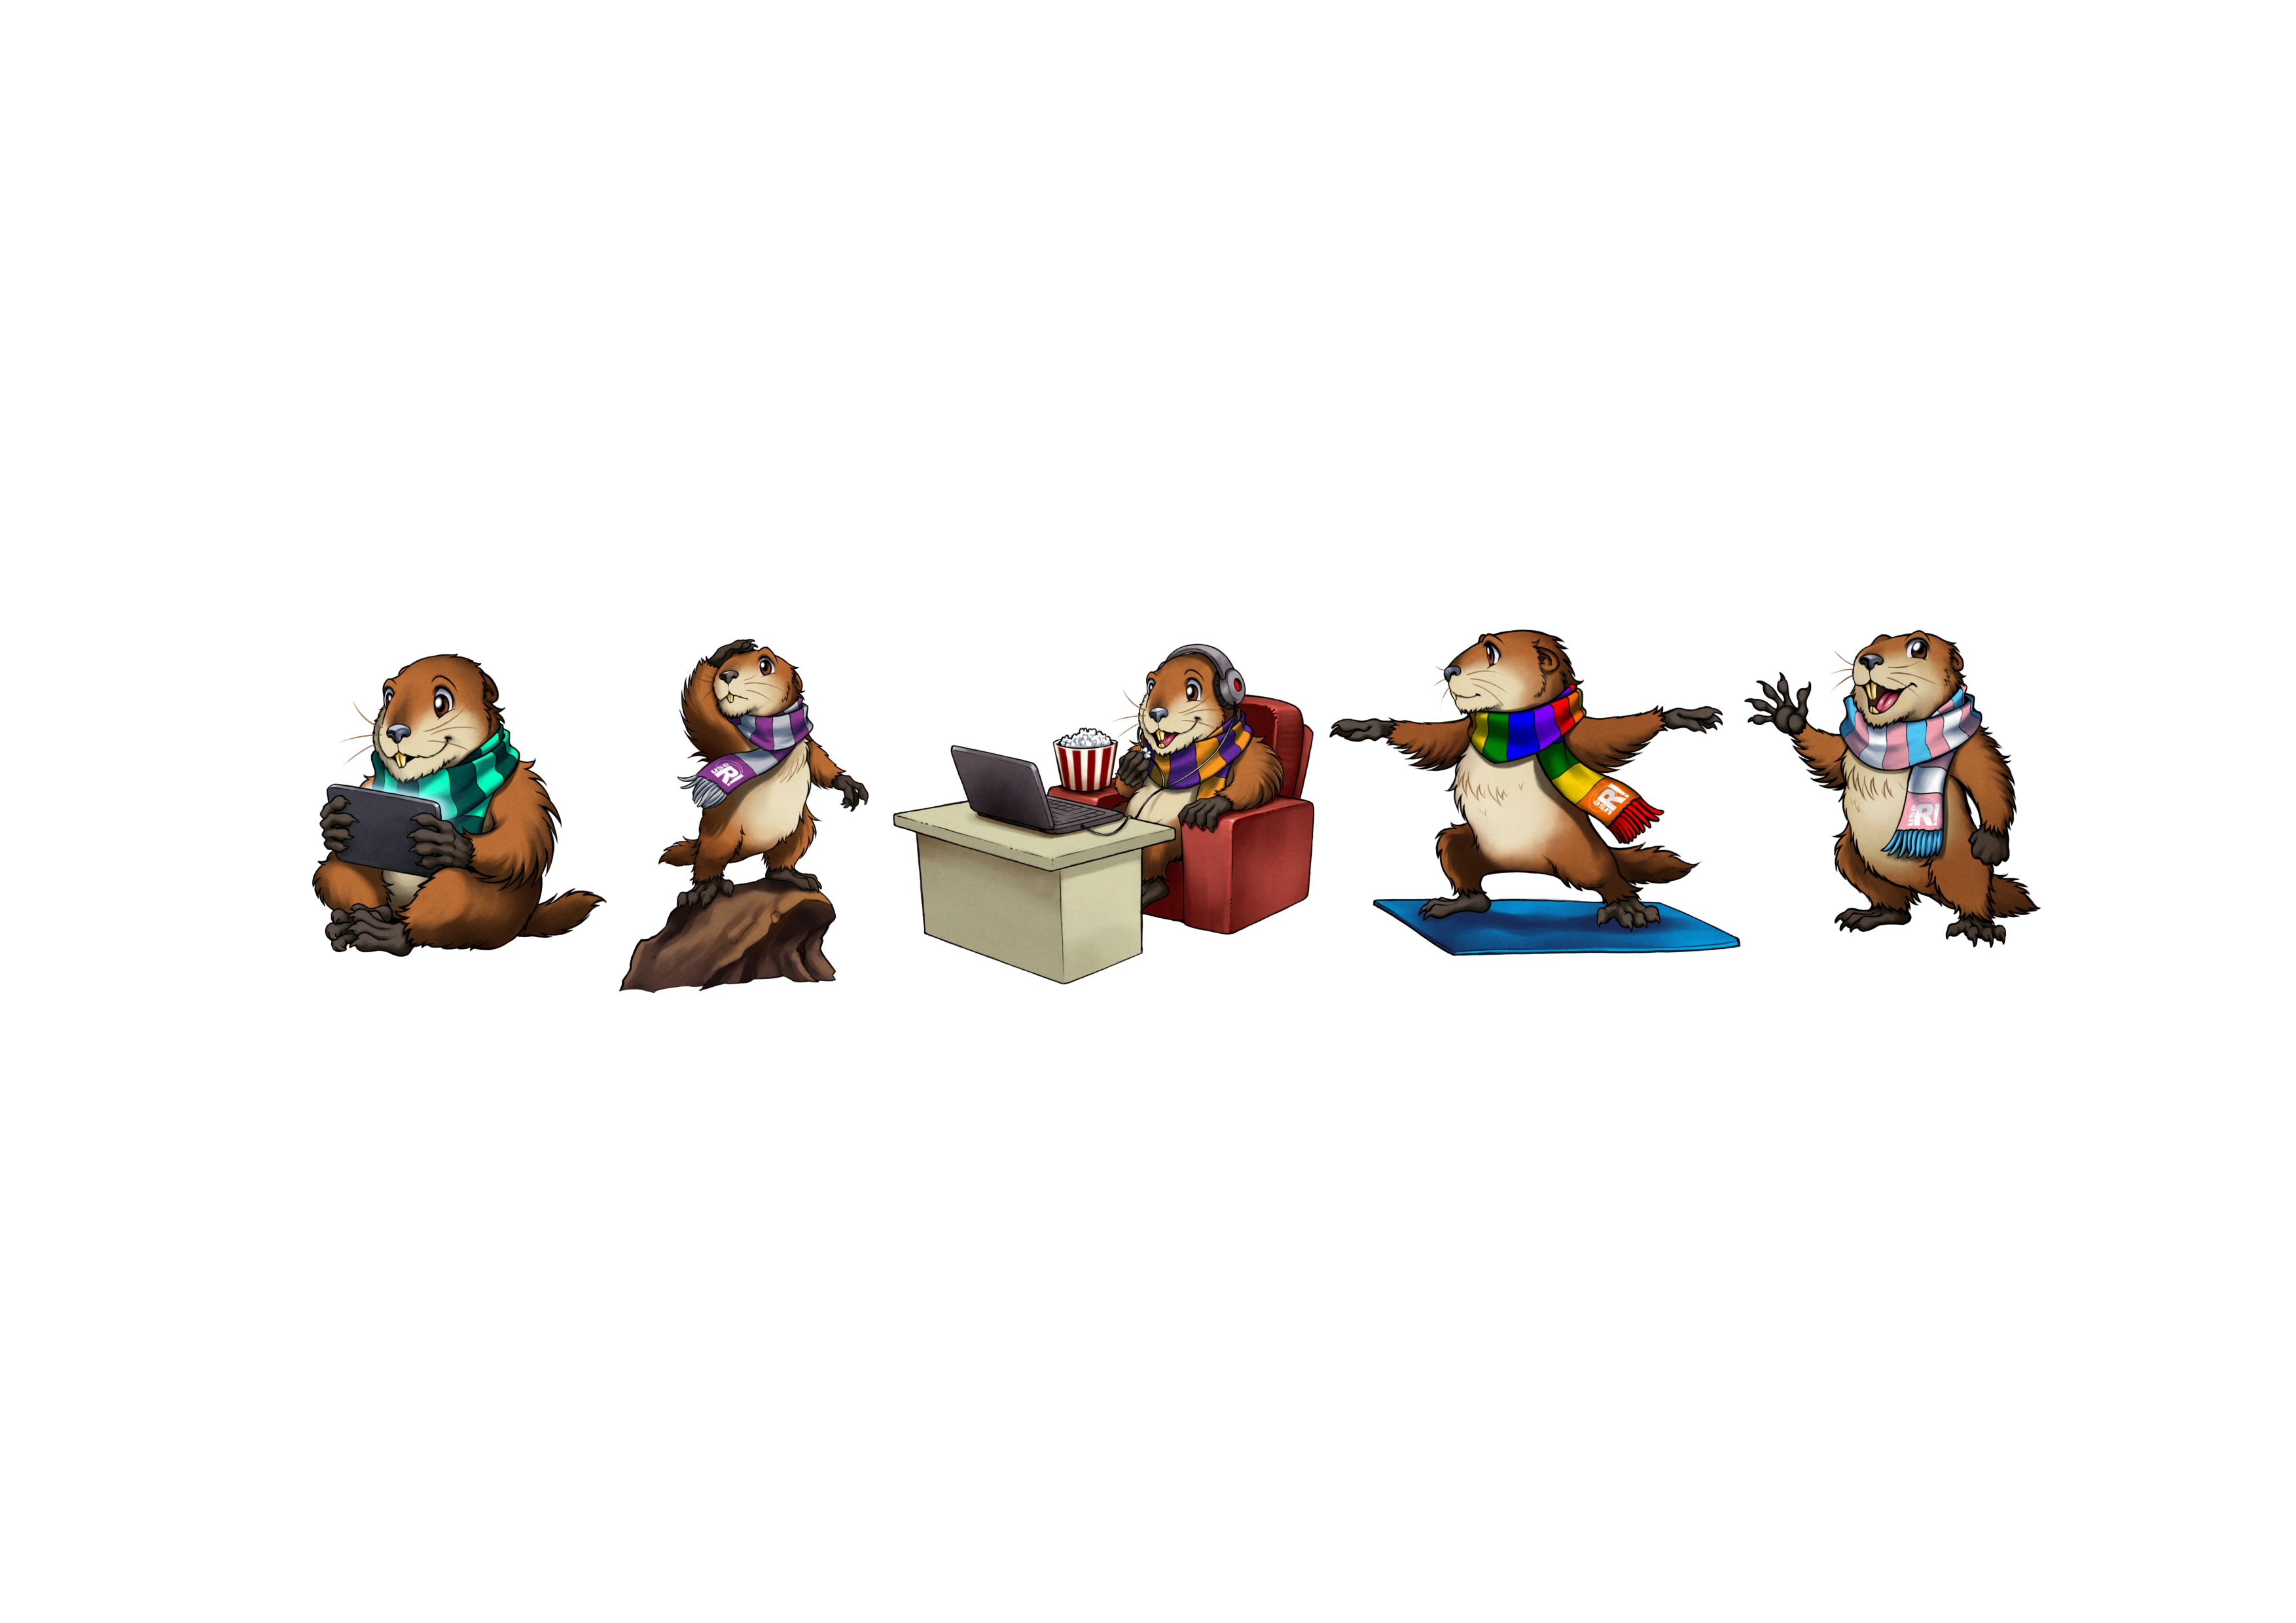
\includegraphics[width=\textwidth]{figs/marmots.pdf}}{
}
\caption{Margot the marmot was the useR! 2021 mascot. To represent the global and inclusive nature of the conference, Margot was drawn using scarves representing the colors of diverse communities of practice that are part of the large R community and specific groups of people we wanted to support explicitly. From left to right: Margot wearing scarves with the colors of MiR (Minorities in R https://mircommunity.com/), R-Ladies https://rladies.org/, AfricaR https://africa-r.org/, and the LGBTQIA+ and transgender communities. Margot was created by Francisco Etchart and is available under a CC-BY-NC-SA license} 
\label{fig:marmots}
\end{figure}
%alt-text for the figure, to be included in the final PDF: Five marmots with colorful scarves. From left to right: a marmot with a dark and light green scarf from the MiR community is watching her tablet, a marmot with the purple and gray scarf for R-Ladies is stepping on a rock and watches the horizon, a marmot with an orange and purple AfricaR scarf is sitting on a couch watching a film on her laptop with popcorn, a yogi marmot with a rainbow LGBTQIA+ scarf does the warrior pose on her blue mat, and finally, a marmot with a scarf with the pink, light blue and white color of the transgender pride flag waves her hand. 

\subsection*{Rule 9: Allocate adequate financial resources to support inclusion goals}
\label{rule_financial}

% Rocío: main idea: Need to budget for inclusive practices.
Allocation of resources to support the diversity and inclusion vision and goals has to be intentional. 
Estimate the costs of these practices and define your priorities in advance (e.g. paying the organizing team, code of conduct training, captioning, accessible software, scholarships).
Consider that an online conference might reduce overall costs (e.g. no rental costs for a physical venue), allowing to redirect the money towards inclusive practices. 
When asking for sponsorship, it might be easier to justify supporting concrete actions towards inclusion than making generic requests for funding.

% Rocío: main idea: help take the burden out of participants for more inclusive participation
When determining the registration rates, the socioeconomic context of participants, their country of origin, and their career status should be taken into account  \cite{sarabipourChangingScientificMeetings2021, andalibPostdocQueueLabour2018, kaplanPostdocNot2012}
(see \cite{canelon2021cost} for an example of conversion rates based on country of origin and career status). 
Resources permitting, enable a `pay what you can' option. You could also aim to have a conference with no registration costs; this is especially true for online events, but bear in mind that free events have a lower attendance rate than paid events \cite{eventbrite_ultimate_2017}. 
Scholarships to attend the in-person component of the conference are an additional way to boost participation of people from marginalized groups, by offering support for travel and lodging expenses.
Design the diversity-related scholarship to be explicit about the groups you want to support, and be transparent about the criteria for evaluation to avoid self-selection (refraining from applying). 
To assign these scholarships, conferences usually ask for cover letters or applications, which can be time-consuming and emotionally demanding. 
Simplifying the process of requesting financial support, especially for 
people who lack the time and resources (e.g. because of family responsibilities) could greatly increase their chances of applying for the support. 
Additional aid for attendees could also be offered—e.g. paying for child care or internet connection services for the virtual component. 
Bear in mind that transferring money internationally could be a cumbersome administrative process and significantly augment the burden of already marginalized groups. Whenever possible, facilitate alternate ways for money transfer (e.g. book flights, hotel reservations, waive conference fees, give gift cards). Depending on the country, services like OpenCollective (https://opencollective.com/) can be very useful to do these transfers. 


\subsection*{Rule 10: Make the conference part of a long-term process for inclusion}
\label{rule_process}

% Rocío: main idea: assess how inclusive was the conference
As conference organizers, one of the key post-conference tasks is to make a final assessment of the achievement of the diversity and inclusion goals. 
You can rely on the diversity indicators defined at the beginning of the planning process (\textbf{Rule 1}). 
It is likely that you will be able to calculate some of your indicators directly from information that you have already collected from your organizing team, speakers, and participants (e.g. countries of origin, or preferred language).
You may have goals concerning how welcomed and included participants felt during the conference, and wonder if your practices translated into real inclusion. Surveys, focal groups, and informal conversations during and after the conference are good ways to collect this type of information and great opportunities to receive feedback from the attendees. 

% Pass the information
The feedback received from the participants and your whole assessment of the conference should be documented and shared with future organizers. 
Gather and do your best to organize all the documentation produced during the organization process—or even after. Timelines, checklists, budgeting tips, email templates, accessibility checks and guidelines, are a few of many resources that can be shared with your conference successors. 
Create a list with contact information of the people of the organizing team, as well as previous and potential speakers—if they agree to share their contact information—, and pass it along.
For conference series, it could be a good idea to create an official document (e.g. a wiki, knowledge base or similar guide, see for instance \cite{sanchez-tapia_user_2021-2}) that can be used and kept up to date by future organizers.
If you are part of a stable meeting committee (overseeing multiple editions), encourage organizers to follow these Rules and set up new standards for inclusion: be explicit on the inclusive spirit of the conference and the practices that future organizers should commit to when publishing the call for conference organization and the selection criteria. 


\section*{Concluding remarks}

This article suggests changes in conference planning towards diversity and inclusion. 
Organizing a conference and implementing inclusive practices are both learning experiences.
As conference organizers ourselves, we started with different levels of clarity about the principles and practices described here, learned many of them together during the organization phase, and learned even more when translating them into ten rules for this paper. 
We hope that they can be useful guidelines to improve diversity and inclusion in your conference, and that you can adapt them, improve them, and share your lessons and experience with as many people as possible. 

Be aware of all the factors that may hinder your efforts for inclusion: systemic discrimination, time or money constraints, geopolitical or public health contexts, or personal issues affecting your organizing team. 
Try to account for these factors as best as you can to set a realistic yet bold vision and goals of diversity and inclusion for the conference.
At the end of the day, even if you do not achieve them at 100\%, striving for them will make you stretch what feels possible and help you make changes you would have otherwise not even attempted to make. 
And most importantly, you would have contributed to a great conference experience for the attendees. 
They will notice the welcoming and inclusive spirit of the conference reflected in the pillar rules and the effort put in every aspect of the conference design. 
Inclusive conferences can have lasting impacts in career paths and create a sense of belonging in the community. 
That is more than enough motivation to make the effort worth it. 


\section*{Authors' contributions}

To list author contributions, we used the high-level contributor roles in the CRediT framework that we considered relevant for this study (project administration, supervision, writing original draft, conceptualization, writing—major reviews and edits, resources, and visualization; \url{http://credit.niso.org}), and an additional category to acknowledge those who shared their own ten simple rules for an inclusive conference without looking at the first draft (i.e. sharing rules).

\begin{itemize}
    \item RJ: Project administration, Supervision, Writing original draft, Conceptualization, Writing--major reviews and edits, Resources, Visualization
    \item AST: Project administration, Supervision, Conceptualization,  Writing--major reviews and edits, Resources, Visualization, Sharing rules
    \item SM: Conceptualization, Writing--major reviews and edits, Resources, Visualization, Sharing rules
    \item YBS: Conceptualization, Writing--major reviews and edits, Resources
    \item HT: Conceptualization, Writing--major reviews and edits, Resources
    \item DHP: Conceptualization, Writing--major reviews and edits, Sharing rules
    \item MB: Conceptualization
    \item BA: Writing--major reviews and edits, Resources, Sharing rules
    \item LH: Writing--major reviews and edits, Resources, Sharing rules
    \item LA: Writing--major reviews and edits, Resources
    \item JPN: Writing--major reviews and edits, Visualization
    \item MAC: Writing--major reviews and edits
    \item FM: Writing--major reviews and edits
    \item RG: Writing--major reviews and edits
    \item NM: Sharing rules
    \item AU: Sharing rules
    \item JC: Sharing rules
    \item AE: Sharing rules
    \item SC: Sharing rules
    \item JR: Conceptualization, Writing--major reviews and edits
\end{itemize}



\section*{Acknowledgments}
The authors of this piece would like to thank every single member of the organizing team of useR! 2021 (\url{https://user2021.r-project.org/about/global-team/}) for their valuable contribution to an inclusive conference experience and the R Foundation for trusting us with the organization of useR! 2021 and supporting us through the process. Special thanks to Saranjeet Kaur and gwynn sturdevant for suggestions to previous versions of the manuscript, and Francisco Etchart for his help with the figures.

Heather Turner was supported by the Engineering and Physical Sciences Research Council [EPSRC EP/V052128/1] during the preparation of this article and by The R Foundation for Statistical Computing during the organization of useR! 2021.


% \nolinenumbers

% % Either type in your references using
% % \begin{thebibliography}{}
% % \bibitem{}
% % Text
% % \end{thebibliography}
% %
% % or
% %
% % Compile your BiBTeX database using our plos2015.bst
\bibliography{community-science}
% % style file and paste the contents of your .bbl file
% % here. See http://journals.plos.org/plosone/s/latex for 
% % step-by-step instructions.
% % % 
% \begin{thebibliography}{10}

% \bibitem{bib1}
% Conant GC, Wolfe KH.
% \newblock {{T}urning a hobby into a job: how duplicated genes find new
%   functions}.
% \newblock Nat Rev Genet. 2008 Dec;9(12):938--950.

% \bibitem{bib2}
% Ohno S.
% \newblock Evolution by gene duplication.
% \newblock London: George Alien \& Unwin Ltd. Berlin, Heidelberg and New York:
%   Springer-Verlag.; 1970.

% \bibitem{bib3}
% Magwire MM, Bayer F, Webster CL, Cao C, Jiggins FM.
% \newblock {{S}uccessive increases in the resistance of {D}rosophila to viral
%   infection through a transposon insertion followed by a {D}uplication}.
% \newblock PLoS Genet. 2011 Oct;7(10):e1002337.

% \end{thebibliography}



\end{document}

